{\fontsize{12pt}{22pt} \textbf{Heavy-Tailed Distribution}\par}

\vspace{5mm}

A distribution is heavy-tailed when there are more chances to get large values. Consequently, the variance is higher and will make the mean misleading as many outliers have high values. Below are p.d.f. (light-tailed and heavy-tailed

\vspace{5mm}

\begin{center}
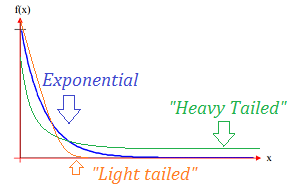
\includegraphics[scale=0.8]{heavy-light-tailed.png}
\end{center}

An real-life example of heavy-tailed distribution is the income in the US.

\vspace{5mm}